\setcounter{equation}{0}
\chapter{Confidence Intervals}
\label{chapterConfidenceIntervals}
\index{Confidence intervals}

\section{Introduction}

We learnt in chapter $\ref{SectionFoundationsOfInference}$
that a point estimate is the best single guess for the numeric value of a parameter and that due to the nature of randomness, a point estimate will likely not be exactly equal to the parameter that it is estimating. Using properties of sampling distributions, we can create an interval around our point estimate which we believe will capture our parameter with a certain level of confidence. This interval is referred to as a \textit{confidence interval} for the parameter of interest.

\begin{definition}[Confidence Interval]
\index{Confidence intervals!Definition}
A confidence interval is a plausible range of values that captures a parameter with a quantified degree of confidence.
\end{definition}

Suppose we are interested in the average mark for STAT*2060 for the current semester. We are 100\% confident that the average mark is between 0 and 100 however this is not useful information as we already know that the average mark must lie between 0 and 100. Using the marks of previous years, we can construct a 95\% interval for the average mark. If it is determined that the average mark lies within 70\% and 80\%, this is much more meaningful as we can state with a high degree of certainty that the average mark is going to lie within a substantially narrow range.\\

In this course, all confidence intervals have the same basic skeleton:

\begin{skeleton}[]
	\begin{equation}
	\text{\large{estimator}} ~\pm~ 	\underbrace{
						\bigg( \parbox[c]{4.25cm}{ \centering value from reference distribution } \bigg)
						\times
						\bigg( \parbox[c]{2.70cm}{ \centering standard error of estimate } \bigg)
						}_{ \text{\large{margin of error} } }
	\end{equation}
\end{skeleton}

\noindent
The value from the reference distribution in the skeleton above 
will be either a value from the standard normal distribution discussed in section $\ref{sectionNormalDistribution}$
or the Student $t$-distribution discussed in section $\ref{sectiontDistribution}$. The margin of error ($MOE$) can be considered as the distance around our estimator in which the true value of the parameter of interest will be found, with a specified level of confidence.

\begin{figure}[H]
\label{figureVisualization of CI}
\begin{center}
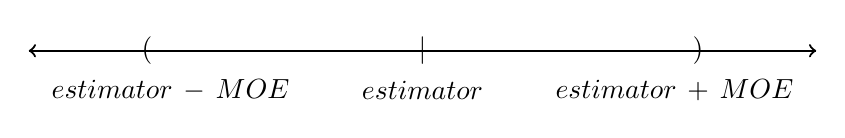
\begin{tikzpicture}
\draw[thick, ->] (-5,0) -- (5,0);
\draw[thick, <-] (-5,0) -- (5,0);
\node at (-3.5,0) {(};
\node at (0,0) {$|$};
\node at (3.5,0) {)};
\node at (0,-0.5) {$estimator$};
\node at (-3.2,-0.5) {$estimator \, - \, MOE$};
\node at (3.2,-0.5) {$estimator \, + \, MOE$};
\end{tikzpicture}
\end{center}
\vspace{-0.60cm}
\caption{Visualization of a confidence interval on the real number line. The margin of error is abbreviated as $MOE$. The estimator is the centre of the interval. The confidence interval consists of all values between the estimator$- MOE$ and the estimator$+ MOE$.}
\end{figure}

The exact form of a confidence interval depends on the information we have and the parameter we are estimating.

\begin{nt}\label{noteOneSidedTwoSidedCIs}
The confidence intervals that we will be constructing are referred to as ``two-sided confidence intervals'' as they provide both a lower and upper bound for a plausible range of values that the parameter of interest can take.\\

One-sided confidence intervals can also be constructed however these types of confidence intervals are not constructed as often as two-sided confidence intervals. One-sided confidence intervals are constructed on rare occasions when a researcher is interested in just a lower or an upper bound for the value of a parameter.
\end{nt}


\section{Interpretation}

We use very specific language when we interpret a confidence interval.

\begin{skeleton}[]
Suppose we construct a $C\%$ confidence interval for some parameter such that $C$ is between 0 and 100. In repeated sampling, we are $C\%$ confident that approximately $C\%$ of the intervals will capture the true value of the parameter.
\end{skeleton}

\begin{figure}
\centering
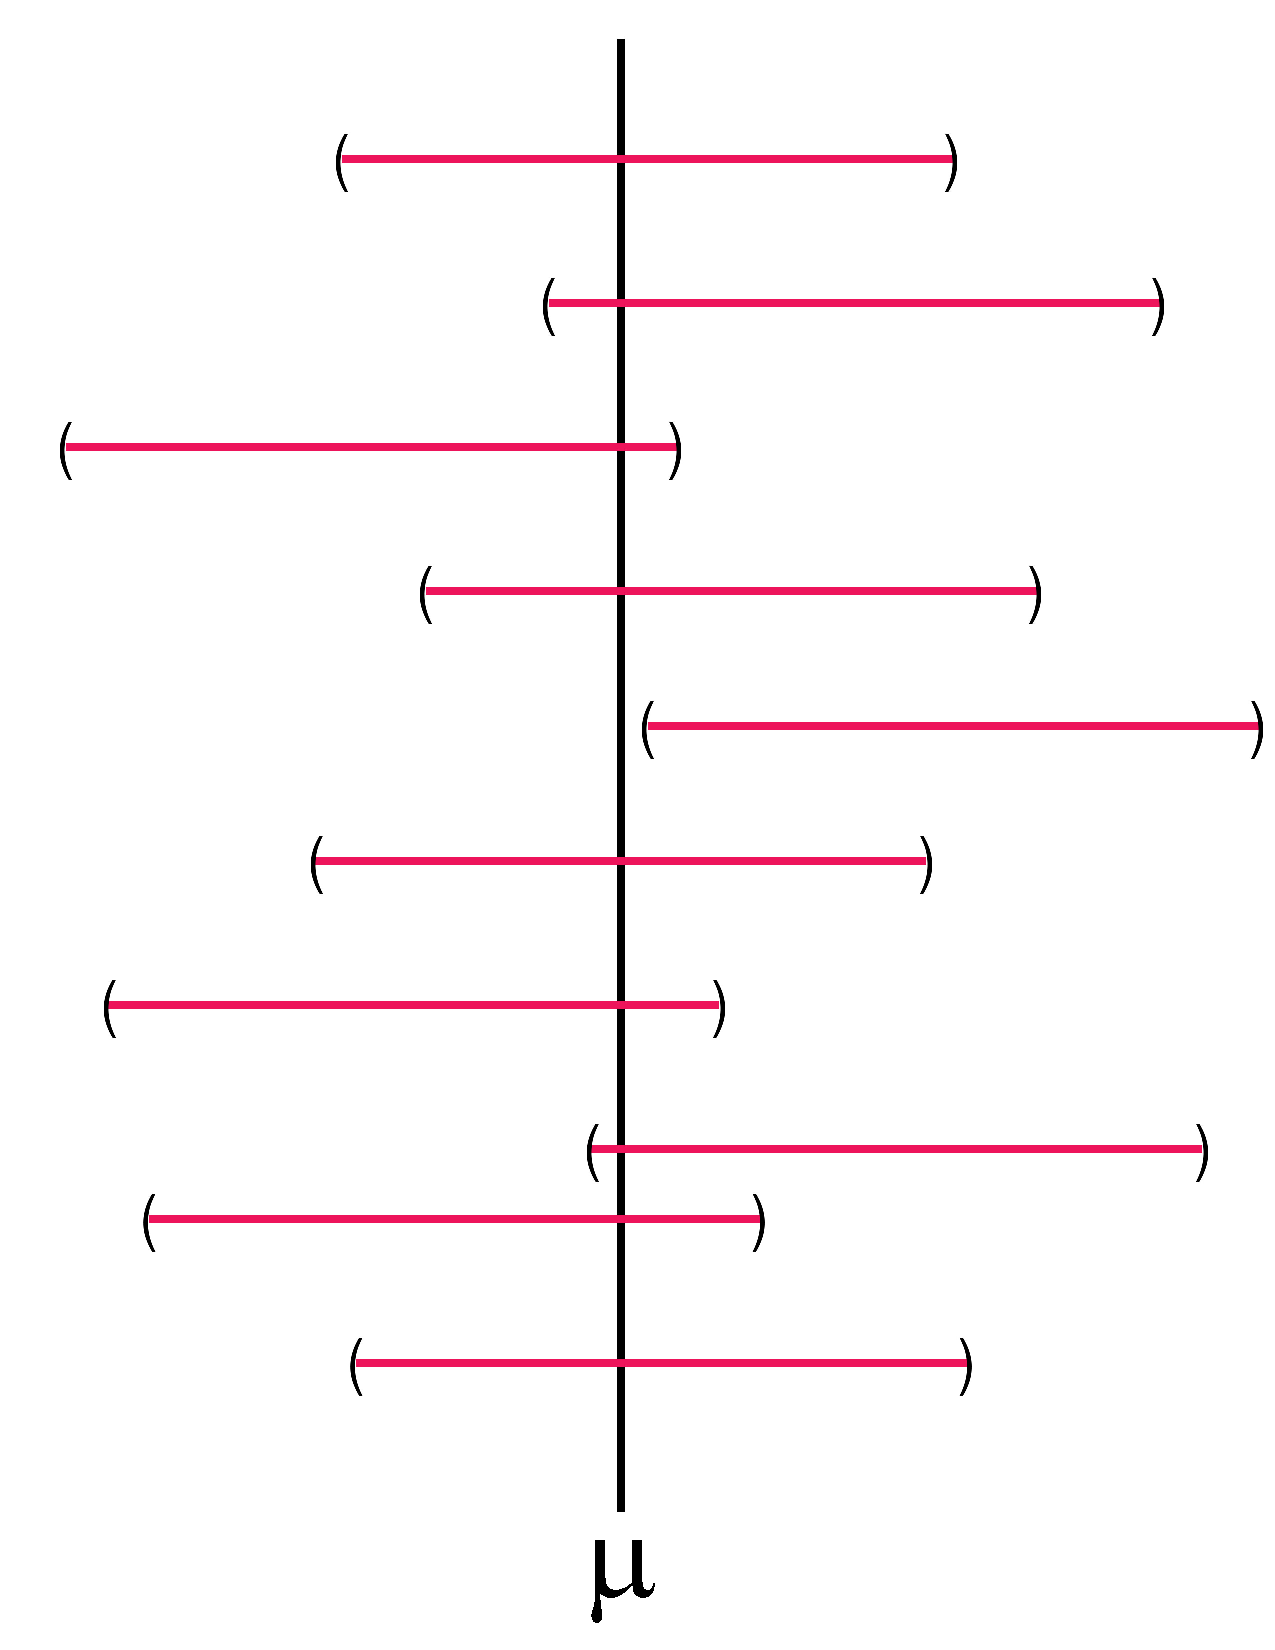
\includegraphics[scale=0.35]{Section6/confidenceinterval.pdf}
\caption{Graphical interpretation of a 90\% confidence interval for $\mu$. Note that 9 of the 10 constructed intervals capture the true value of $\mu$.}
\end{figure}

By this we mean that if we constructed several $C\%$ confidence intervals using different samples (with or without replacing the units), then we should expect approximately $C\%$ of these intervals to capture the parameter of interest. For example suppose we construct 1000 95\% confidence intervals for the population mean $\mu$. We would expect approximately 95\% of these 1000 intervals
(i.e. $95\% \times 1000 = 950$) to actually capture $\mu$.

\begin{nt}
A more intuitive but equivalent interpretation is to state that we are $C$\% confident that our target parameter is inside the interval constructed.
\end{nt}

It is incorrect to state that there is a $C\%$ probability that 
the interval we constructed contains the parameter of interest.
Recall from assumption $\ref{assumptionInferenceParameter}$ that we assume that the value of a parameter is fixed. Therefore when we construct a confidence interval, the interval either contains the parameter or it does not.


\section{One Sample Confidence Intervals}
\index{Confidence intervals!One sample}

\subsection{On the Mean}
\index{Confidence intervals!On the mean}

\subsubsection{When $\sigma$ is Known}


When we know the population standard deviation $\sigma$, we can construct a confidence interval for $\mu$ in the following manner.

\begin{ci}[Confidence Interval on $\mu$ when $\sigma$ is Known]
A $(100 - \alpha)\%$ confidence interval on $\mu$ when $\sigma$ is known
is 
\begin{equation}\label{eqnCISigmaKnown}
\bar{x}	~\pm~	z_{\alpha / 2}  \bigg( \frac{\sigma}{ \sqrt{n} } \bigg)
\end{equation}
\end{ci}

\noindent
The $z_{\alpha/2}$ value is obtained from standard normal tables. The standard error in $\ref{eqnCISigmaKnown}$ is $ \frac{\sigma}{ \sqrt{n} }$
and the margin of error is $z_{\alpha / 2} \bigg( \frac{\sigma}{ \sqrt{n} } \bigg)$.


\begin{example}
\label{exampleCiOnMuSigmaKnown}
Corporation $A$'s closing stock prices over the past year are assumed to be approximately normally distributed. 10 closing stock prices were sampled from the past year:
\begin{center}
\begin{tabular}{cccccccccc}
49.43 & 56.47 & 52.76 & 56.34 & 47.67 & 40.73 & 49.55 & 56.12 & 37.32 & 53.68
\end{tabular}
\end{center}
The corporation is interested in estimating $\mu$, the true mean closing stock price over the past year.
If the true standard deviation of Corporation A stock prices is known to be $\sigma=10$, construct a 95\% confidence interval for $\mu$.

\hfill\\
{\emph{\textbf{\underline{Solution:}}}}\\


First, we find $\bar{x}$.
\begin{align*}
\bar{x} &= \sum_{i=1}^{n} \frac{x_i}{n} = \sum_{i=1}^{10} \frac{x_i}{10} \\
			&=\frac{49.43+56.47+ 52.76 + 56.34 + \hdots + 37.32 + 53.68}{10}\\
			&=50
\end{align*}

Second, we find the margin of error.
\[\text{Margin of Error}~=z_{\alpha/2} \left(\frac{\sigma}{\sqrt{n}}\right) \]
For a 95\% confidence interval, $\alpha = 0.05$ and $z_{\alpha/2} = z_{0.025} = 1.96$.
\begin{align*}
\Rightarrow \text{Margin of Error}= 1.96 \left( \frac{10}{\sqrt{10}} \right) =1.96 \times 3.16 = 6.19
\end{align*}
The 95\% confidence interval for $\mu$ when $\sigma=10$ is 
\begin{align*}
\bar{x} \pm z_{\alpha/2} \left(\frac{\sigma}{\sqrt{n}}\right) = 50 \pm 6.19= (43.81,~56.19)
\end{align*}

\end{example}







\subsubsection{When $\sigma$ is Unknown}
When we do not know the population standard deviation $\sigma$,
we estimate it with the sample standard deviation $s$ and
construct a confidence interval for $\mu$ in the following manner.

\begin{ci}[Confidence Interval on $\mu$ when $\sigma$ is Unknown]\label{CIonMuSigmaNotKnown}
A $(100 - \alpha)\%$ confidence interval on $\mu$ when $\sigma$ is unknown
is
\begin{equation}\label{eqnCISigmaNotKnown}
\bar{x}	~\pm~	t_{(\alpha / 2, ~n-1)}  \bigg( \frac{s}{ \sqrt{n} } \bigg)
\end{equation}
\end{ci}

\noindent
The $t_{(\alpha/2,~n-1)}$ value in $\ref{eqnCISigmaNotKnown}$ 
is obtained from the $t-$distribution by referring to the $t-$tables with $n-1$ degrees of freedom. The standard error in $\ref{eqnCISigmaNotKnown}$ is
$s/\sqrt{n}$ and the margin of error is $t_{(\alpha / 2, ~n-1)}  (s / \sqrt{n})$.


\begin{example}
\label{exampleCiOnMuSigmaUnknown}
Corporation A's closing stock prices over the past year are assumed to be approximately normally distributed. 10 closing stock prices were sampled from the past year:
\begin{center}
\begin{tabular}{cccccccccc}
49.43 & 56.47 & 52.76 & 56.34 & 47.67 & 40.73 & 49.55 & 56.12 & 37.32 & 53.68
\end{tabular}
\end{center}
The corporation is interested in estimating $\mu$, the true mean closing stock price over the past year.
If the true standard deviation of Corporation A stock prices is unknown, construct a 95\% confidence interval for $\mu$.


\hfill\\
{\emph{\textbf{\underline{Solution:}}}}\\


Since we do not know $\sigma$, we must estimate it using $s$. 
\begin{align*}
s^2 &= \sum_{i=1}^{n} \frac{(x_i - \bar{x})^2}{n-1} = \sum_{i=1}^{10} \frac{(x_i - 50)^2}{9}\\
	   &= \frac{(49.43-50)^2}{9} + \frac{(56.47-50)^2}{9} + \frac{(52.76-50)^2}{9} + \hdots + \frac{(53.68-50)^2}{9} \\
	   &= \frac{0.32+41.86+ 7.62+ 40.20+5.43+ 85.93+  0.20+ 37.45+ 160.78+  13.54}{9}\\
	   &= 43.704 \\
\Rightarrow s &= \sqrt{s^2} = \sqrt{43.704} = 6.61 
\end{align*}
To calculate the margin of error, we can no longer use $z_{\alpha/2}$ as $\sigma$ is unknown. Therefore we use $t_{\alpha/2,~n-1}$. 
\[ \text{Margin of Error}= t_{(\alpha/2,~n-1)} \left(\frac{s}{\sqrt{n}}\right)\]
$t_{\alpha/2,~n-1}$ is the probability that $t$ is greater than $t_{\alpha/2}$ or less than $-t_{\alpha/2}$ for a t-distribution with $n-1$ degrees of freedom. Using our t-distribution table, we find that $t_{0.025,9}$ is 2.26.
\[ \Rightarrow \text{Margin of Error}=2.26 \left( \frac{6.61}{\sqrt{10}} \right) = 2.26 \times 2.09 = 4.72\]
The 95\% confidence interval for $\mu$ when $\sigma$ is unknown is
\[ \bar{x} \pm t_{(\alpha/2,~n-1)} \left( \frac{s}{\sqrt{n}} \right) = 50 \pm 4.72 = (45.28,~54.72)\]

\end{example}








\subsection{On a Proportion}
\index{Confidence intervals!On a proportion}

When we are interested in constructing a confidence interval for a proportion,
we use the sample proportion $\hat{p}$.

\begin{ci}[Confidence Interval on a Proportion]
A $(100 - \alpha)\%$ confidence interval on $p$ is
\begin{equation}\label{eqnCIonProp}
\hat{p}	~\pm~	z_{\alpha / 2}  \sqrt{ \frac{ \hat{p} (1-\hat{p}) }{n} }
\end{equation}
\end{ci}
\noindent
The standard error in $\ref{eqnCIonProp}$ is
$\sqrt{ \frac{ \hat{p} (1-\hat{p}) }{n} }$
and the margin of error is 
$z_{\alpha / 2}  \sqrt{ \frac{ \hat{p} (1-\hat{p}) }{n} }$.



\begin{example}
\label{exampleCiOnP}
Corporation A's closing stock prices over the past year are assumed to be approximately normally distributed. 10 closing stock prices were sampled from the past year:
\begin{center}
\begin{tabular}{cccccccccc}
49.43 & 56.47 & 52.76 & 56.34 & 47.67 & 40.73 & 49.55 & 56.12 & 37.32 & 53.68
\end{tabular}
\end{center}

Suppose Corporation A is interested in the proportion of closing stock prices during the past year that were greater than fifty dollars. Using the information provided, construct a 95\% confidence interval for $p$. 


\hfill\\
{\emph{\textbf{\underline{Solution:}}}}\\


First we need to find $\hat{p}$. 
\begin{align*}
\hat{p} = \frac{\text{number of closing stock prices}>~\text{\$50 in sample}}{n} = \frac{5}{10} = 0.5
\end{align*}
From Example $\ref{exampleCiOnMuSigmaKnown}$, we know that $z_{\alpha/2}$ is $z_{0.025}=1.96$ for a 95\% confidence interval. The margin of error is then
\begin{align*}
\text{Margin of Error} &= z_{\alpha/2} \sqrt{\frac{\hat{p}(1-\hat{p})}{n}}
									= 1.96 \sqrt{\frac{0.5 (1-0.5)}{10}}
									= 1.96 \times 0.158
									= 0.31
\end{align*}
The 95\% confidence interval for $p$ is
\[ \hat{p} \pm z_{\alpha/2} \sqrt{\frac{\hat{p}(1-\hat{p})}{n}} = 0.50 \pm 0.31 = (0.19, 0.81) \]

\end{example}




\subsection{Assumptions}
\index{Confidence intervals!Assumptions}


\begin{assumptions}[Assumptions for One-Sample Confidence Intervals for $\mu$]
In order to construct confidence intervals on the population mean $\mu$, 
the following assumptions must be met in order for their construction to be valid.

\begin{enumerate}
\item Data is from a random sample of a large population.			
\item Observations in the sample are independent of each other.	
\item If the sample size is small, the population distribution must be approximately normal. For large sample sizes, the population does not need not be approximately normal due the effect of the Central Limit Theorem (refer to section $\ref{sectionCLT}$).
\end{enumerate}

\end{assumptions}





\begin{assumptions}[Assumptions for One-Sample Confidence Intervals for $p$]\label{assumptionsOnP}
\index{Confidence intervals!Assumptions}

In order to construct confidence intervals on the population proportion $p$, 
the following assumptions must be met in order for their construction to be valid.

\begin{enumerate}
\item Data is from a random sample of a large population.
\item Observations in the sample are independent of each other.
\item	$np \geq 10$ and $n(1-p) \geq 10$.	\label{assumpSampleSizeForP}
\end{enumerate}

\end{assumptions}

\begin{nt}
Assumption $\ref{assumpSampleSizeForP}$ in $\ref{assumptionsOnP}$
can be tested by verifying whether $\hat{p} \geq 10$ and $n (1 - \hat{p}) \geq 10$\
\end{nt}



\begin{example}
Are the assumptions for the confidence intervals constructed in 
examples $\ref{exampleCiOnMuSigmaKnown}$, $\ref{exampleCiOnMuSigmaUnknown}$  and $\ref{exampleCiOnP}$ met?

\hfill\\
{\emph{\textbf{\underline{Solution:}}}}\\

In order to construct confidence intervals for $\mu$ and $p$ observations in the sample must be independent of each other. Our sample contains daily closing stock prices from the past year. It is unlikely that these closing prices are independent. If a stock performs poorly today, it is likely that the price will continue to drop tomorrow. Alternatively, if a stock performs well today, it is likely that the price will continue to rise tomorrow. \\

In order to construct a confidence interval for $p$, the following must hold:
\begin{enumerate}[1.]
\item $n\hat{p} \geq 10$
\item $n(1-\hat{p}) \geq 10$
\end{enumerate} 

However, for $n=10$ and $\hat{p}=0.5$,
\begin{align*}
n \hat{p} &= 10 \times 0.5 = 5 < 10 \\
n(1-\hat{p}) &= 10(1-0.5) = 10 \times 0.5 = 5 < 10 
\end{align*}

The assumptions are not met and therefore the confidence intervals are not valid.

\end{example}


\section{Two Sample Confidence Intervals}
\index{Confidence intervals!Two sample}

We are often interested in determining whether there is a significant difference in the parameters of two populations. In such cases we draw independent samples from each population and construct confidence intervals for the difference between the parameters of interest.

\subsection{On a Difference of Two Means}
\index{Confidence intervals!On a difference of two means}

Consider two populations. One population has a mean $\mu_{1}$ and standard deviation $\sigma_{1}$ and the other population has mean $\mu_{2}$ and standard deviation $\sigma_{1}$. We draw a sample of size $n_1$ from the first population and calculate the sample mean, standard deviation and size 
of the sample drawn from this population. We draw an independent sample of size $n_2$ from the second population and calculate the same statistics.

\begin{figure}[H]
\begin{center}
\begin{tikzpicture}[thick,scale=1.5, every node/.style={scale=1.25}]

\footnotesize
\draw[fill=oiB] (1,3)
ellipse (2.25 and 0.5);

\node[draw=none] at (1,3.20) {Population 1};
\node[draw=none] at (1,2.80) {$\mu_{1}, ~\sigma_{1}$};%,  ~p_{1}$};

\draw[->] (1,2.25) -- (1, 1.00);

\draw[fill=oiB7] (1,0.25)
ellipse (1.75 and 0.50);
\node[draw=none] at (1.00, 0.45) {Sample 1};
\node[draw=none] at (1.00, 0.05) {$\bar{x}_{1}, ~s_{1},~n_{1}$};%,~\hat{p}_{1}$};

\draw[fill=oiG6] (7,3)
ellipse (2.25 and 0.5);

\node[draw=none] at (7,3.20) {Population 2};
\node[draw=none] at (7,2.80) {$\mu_{2}, ~\sigma_{2}$};%,  ~p_{2}$};


\draw[->] (7,2.25) -- (7, 1.00);

\draw[fill=oiG9] (7,0.25)
ellipse (1.75 and 0.50);
\node[draw=none] at (7.00, 0.45) {Sample 2};
\node[draw=none] at (7,0.05) {$\bar{x}_{2}, ~s_{2},~n_{2}$};%,~\hat{p}_{2}$};

\end{tikzpicture}
\end{center}
\caption{Sampling from two populations to construct a confidence interval on a difference of means.}
\end{figure}

Suppose we are interested in the difference in average salary between males and females at the management level in a certain region. The two populations of interest all males and all females in at the management level in this region. Let $\mu_{1}$ represent the average salary of all males at the management level and $\mu_{2}$ represent the average salary of all females at the management level. The parameter of interest is $\mu_{1} - \mu_{2}$. If both the lower and upper bounds of interval $\mu_{1} - \mu_{2}$ are greater than $0$, the interval provides evidence that $\mu_{1} - \mu_{2} > 0$ 
which therefore suggests that $\mu_{1} > \mu_{2}$. In other words, it provides evidence that the average salary of males is greater than the average salary of females at the management level in a certain region. If both the lower and upper bounds of interval $\mu_{1} - \mu_{2}$ are less than $0$, the interval provides evidence that $\mu_{1} < \mu_{2}$. If the interval $\mu_{1} - \mu_{2}$ contains 0 then it is plausible that $\mu_{1} - \mu_{2} = 0$ which suggests that $\mu_{1} = \mu_{2}$. In other words, it provides evidence that the average salary of males is equal to the average salary of females at the management level in the region.\\

We could have also let  $\mu_{1}$ represent the average salary
of all females at the management level and $\mu_{2}$ represent the average salary of all males and also constructed this confidence interval. We just have to be careful about the manner in which we interpret the
confidence interval we constructed. In the end however our conclusion would be the same.

\subsubsection{When $\sigma_{1}$ and $\sigma_{2}$ are Known} 


\begin{ci}[Confidence Interval on $\mu_{1} - \mu_{2}$ when $\sigma_{1}$ and $\sigma_{2}$ are Known]
A $(100 - \alpha)\%$ confidence interval on $\mu_{1} - \mu_{2}$ 
when $\sigma_{1}$ and $\sigma_{2}$ are both known is

\begin{equation}
\label{eqnCiTwoSampleMeanSigmasKnown}
\big(\bar{x}_{1}	 - \bar{x}_{2}\big)	~\pm~		z_{\alpha / 2}  
\sqrt{ \displaystyle\frac{\sigma_{1}^{2} }{ n_{1} }  +  \frac{\sigma_{2}^{2} }{ n_{2}  }  }
\end{equation}

\end{ci}

\begin{example}
Company $A$ is worried about their stock market performance during different periods of the business cycle. It wants to determine whether there is a significant difference in the daily return of their stock in recessionary years vs. boom years. Recessionary and boom periods were identified over the past ten years and a sample of ten daily returns was collected for both periods. 

\begin{center}
\begin{tabular}{c|c|c|c|c|c|c|c|c|c|c}
\def\arraystretch{2}
Period & \multicolumn{10}{c}{Daily Return (\%)} \\ 
\hline
Boom & 26.87& 30.92 &25.82& 37.98& 31.65& 25.90 &32.44 &33.69& 32.88& 28.47 \\ 
\hline 
Recession & 22.68  & 5.85&  -9.32& -33.22&  16.87  &-0.67 & -0.24 & 14.16&  12.32&   8.91
\end{tabular} 
\end{center}

If it is known that the standard deviation of daily returns in boom years is $\sigma_B = 40\%$ and the standard deviation of deviations in recessionary years is $\sigma_R=30\%$, construct a 95\% CI for the difference in mean daily returns, $\mu_B - \mu_R$.


\hfill\\
{\emph{\textbf{\underline{Solution:}}}}\\


We start by finding $\bar{x}_B$ and $\bar{x}_R$. 

\begin{align*}
\bar{x}_B 	&= \sum_{i=1}^{n_B} \frac{x_i}{n_B}=\sum_{i=1}^{10} \frac{x_i}{10} \\
			&= \frac{26.87+30.92+25.82+\hdots+32.88+28.47}{10} \\
			&= \frac{306.62}{10}=30.66
\end{align*}
\begin{align*}
\bar{x}_R	&= \sum_{i=1}^{n_R} \frac{x_i}{n_R}=\sum_{i=1}^{10} \frac{x_i}{10} \\
			&= \frac{22.68+5.85-9.32+\hdots+12.32+8.91}{10}\\
			&= \frac{37.34}{10} = 3.73
\end{align*}

\[ \Rightarrow \bar{x}_B - \bar{x}_R = 30.66-3.73 = 26.93\]


$z_{\alpha/2}=1.96$ for a confidence level of 95\%. $n_B=n_R=10$ as we sampled 10 daily returns for each period. The margin of error is then
\begin{align*}
\text{Margin of Error} 	&= z_{\alpha/2} \sqrt{\frac{\sigma_B^2}{n_B}+\frac{\sigma_R^{2}}{n_R}} \\
						&= 1.96 \sqrt{\frac{40^2}{10}+\frac{30^2}{10}} \\
						&= 1.96 \sqrt{160+90} = 1.96 \times 15.81 = 30.99
\end{align*}

Putting everything together, a 95\% confidence interval for $\mu_B-\mu_R$ is
\[
(\bar{x}_B - \bar{x}_R) \pm z_{\alpha/2} \sqrt{\frac{\sigma_B^2}{n_B}+\frac{\sigma_R^{2}}{n_R}} = 26.93 \pm 30.99 = (-4.06,57.92)
\]
The 95\% confidence interval contains 0 and therefore suggests that there is evidence that the mean daily return during boom periods does not differ from the mean daily return during recessionary periods. 
\end{example}









\subsubsection{When $\sigma_{1}$ and $\sigma_{2}$ are Unknown} 

We now consider the more realistic case where both population standard deviations are both unknown. This case is broken down into two sub-cases which are when $\sigma_{1}$ and $\sigma_{2}$ are assumed or known to be unequal and when $\sigma_{1}$ and $\sigma_{2}$ are assumed or known to be unequal. There are statistical tests available to test whether the population standard deviations are equal or not but these tests are beyond the scope of this course. 
However since this is an introductory text, we will consider that we either know or at least we can assume that the population standard deviations are equal or different based on additional information
available from the study or expert knowledge in the area of interest. If the population standard deviations are in fact equal, the sample standard deviations will typically be reflective of this (i.e. if $\sigma_{1} = \sigma_{2}$, we would expect $s_{1} \approx s_{2}$).

\begin{nt}
In general, do not automatically assume that $\sigma_{1} = \sigma_{2}$.
\end{nt}


\begin{rules}[Rule of Thumb for Testing Equality of Variances]
There is a crude rule of thumb that can be implemented
quickly to test whether we can assume equality of variances or not.
Divide the larger sample standard deviation by the smaller sample standard deviation. If the resulting value is greater than or equal to two, we should not assume $\sigma_{1}  = \sigma_{2}$. Formally,

\begin{equation}
\frac{ \max(s_{1}, s_{2}) }{ \min(s_{1}, s_{2}) } \geq 2	
~~ \longrightarrow ~~ \text{Do \underline{not} assume }  \sigma_{1}  = \sigma_{2}
\end{equation}
\end{rules}

\paragraph{When $\sigma_{1} \neq \sigma_{2}$}
\noindent
If the population variances are not equal we construct 
a confidence interval in the following manner.



\begin{ci}[Confidence Interval on $\mu_{1} - \mu_{2}$ when $\sigma_{1} \neq \sigma_{2}$]
\label{ciOnDiffMeanSigmasNotEqual}
A $(100 - \alpha)\%$ confidence interval on $\mu_{1} - \mu_{2}$ when $\sigma_{1} \neq \sigma_{2}$
is
\begin{equation}\label{eqnCITwoSampleSigmasUnknownUnequal}
\big(\bar{x}_{1}	 - \bar{x}_{2}\big)	~\pm~		t_{(\alpha / 2, ~d)} 
\sqrt{ \displaystyle\frac{s_{1}^{2} }{ n_{1} }  +  \frac{s_{2}^{2} }{ n_{2}  }  }
\end{equation}
where a conservative estimate of $d$ is given by $d = \min(n_{1} - 1, ~n_{2} - 1)$.
\end{ci}

\noindent
\index{Welch-Satterthwaite method}
Confidence interval $\ref{ciOnDiffMeanSigmasNotEqual}$ 
is also known as the \textit{Welch-Satterthwaite} method or \textit{Welch's} method.

\begin{nt}
We stated a conservative estimate of the degrees of freedom, $d$,
for confidence interval $\ref{ciOnDiffMeanSigmasNotEqual}$. 
A more accurate calculation of the degrees of freedom is given by:
	\begin{equation}
	d = 	\displaystyle\frac{  \bigg( \displaystyle\frac{ s_{1}^2 }{ n_{1} } + \frac{ s_{2}^2 }{ n_{2} } \bigg)^{2}  }{
		\displaystyle\frac{ \big(  s_{1}^{2} / n_{1}  \big)^{2}  }{ n_{1} - 1}
		+
		\displaystyle\frac{ \big( s_{2}^{2} / n_{2 } \big)^{2}  }{n_{2} - 1}
		}
	\end{equation}
With this calculation of $d$, we will typically not get a whole number and we round down to the nearest integer.
\end{nt}

\begin{example}
Company $A$ is worried about their stock market performance during different periods of the business cycle. It wants to determine whether there is a significant difference in the daily return of their stock in recessionary years vs. boom years. Recessionary and boom periods were identified over the past ten years and a sample of ten daily returns was collected for both periods. 

\begin{center}
\begin{tabular}{c|c|c|c|c|c|c|c|c|c|c}
\def\arraystretch{2}
Period & \multicolumn{10}{c}{Daily Return (\%)} \\ 
\hline %\hline
Boom & 26.87& 30.92 &25.82& 37.98& 31.65& 25.90 &32.44 &33.69& 32.88& 28.47 \\ 
\hline 
Recession & 22.68  & 5.85&  -9.32& -33.22&  16.87  &-0.67 & -0.24 & 14.16&  12.32&   8.91
\end{tabular} 
\end{center}

If the standard deviation of daily returns is unknown for both periods and they are assumed to be different, construct a 95\% CI for the difference in mean daily returns, $\mu_B - \mu_R$.


\hfill\\
{\emph{\textbf{\underline{Solution:}}}}\\


It is known that $\bar{x}_B = 30.66$ and $\bar{x}_R=3.73$ from previous examples. In order to construct the 95\% confidence interval when $\sigma_B$ and $\sigma_R$ are unknown, we first find $s^2_B$ and $s^2_R$. 

\begin{align*}
s^{2}_B &= \sum_{i=1}^{n_B} \frac{(x_i - \bar{x}_B)^2}{n_B-1} \\
		&= \sum_{i=1}^{10}\frac{ (26.87-30.66)^2+(30.92-30.66)^2+\hdots + (28.47-30.66)^2}{9} \\
		&= \frac{14.38+ 0.07+ \hdots + 4.80}{9} \\
		&= 15.24
\end{align*}
\begin{align*}
s^{2}_R &= \sum_{i=1}^{n_R} \frac{(x_i - \bar{x}_R)^2}{n_R-1} \\
		&= \sum_{i=1}^{10}\frac{ (22.68-3.73)^2+(5.85-3.73)^2+\hdots + (8.91-3.73)^2}{9} \\
		&= \frac{358.95+ 4.48+ \hdots + 26.79}{9} \\
		&= 257.38
\end{align*} 

We use the conservative estimate of $d$,
\[ d= min(n_B-1,n_R-1) = 9 \]
Using our t-distribution table we find $t_{(0.025, 9)} = 2.26$. Our margin of error is then
\begin{align*}
\text{Margin of Error} &= t_{(0.025, 9)} \sqrt{\frac{s_B^2}{n_B}+\frac{s_R^2}{n_R}} \\
&= 2.26 \sqrt{ \frac{15.24}{10}+\frac{257.38}{10}} = 2.26 \sqrt{1.52+25.74} = 2.26 \times 5.22 \\
&= 11.80
\end{align*}
Putting it all together, a 95\% confidence interval for $\mu_B-\mu_R$ is
\[ (\bar{x}_B - \bar{x}_R) \pm t_{(\alpha/2,d)} \sqrt{\frac{s_B^2}{n_B} + \frac{s_R^2}{n_R}} = 26.93 \pm 11.80 = (15.13,38.73)\]

The 95\% confidence interval does not contain 0 and therefore suggests that there is evidence that the mean daily return during boom periods differs from the mean daily return during recessionary periods. Furthermore, since the interval was constructed as $\bar{x}_B - \bar{x}_R$ and both the lower and upper bounds are positive, this suggests that the mean daily return is greater during boom periods than recessionary periods. 

\end{example}


\paragraph{When $\sigma_{1} = \sigma_{2}$}

\noindent
If the population variances are equal we construct 
a confidence interval in the following manner.

\begin{ci}[Confidence Interval on $\mu_{1} - \mu_{2}$ when $\sigma_{1} = \sigma_{2}$]
\label{ciOnDiffMeanSigmasNotEqual}
A $(100 - \alpha)\%$ confidence interval on $\mu_{1} - \mu_{2}$ when $\sigma_{1} = \sigma_{2}$ is 
\begin{equation}
\big(\bar{x}_{1}	 - \bar{x}_{2}\big)	~\pm~		t_{(\alpha / 2, ~n_{1}+n_{2}-2)}  
 \displaystyle \sqrt{ s_{p}^{2} \bigg( \frac{1}{n_{1}}  +  \frac{1}{n_{2}}  \bigg) }
\end{equation}
where
\begin{equation}\label{equationPoolSampleVariance}
s_{p}^{2} =  \frac{ (n_{1} - 1) s_{1}^{2} + (n_{2} - 1) s_{2}^{2} }{ n_{1} + n_{2} - 2 }
\end{equation}
\end{ci}

%\begin{nt}
%$s_{p}^{2}$ is referred to as the pooled sample variance. It is the two-sample average of the variances. $s_{p}=+/sqrt{s_{p}^2}$ is referred to as the pooled sample standard deviation.
%\end{nt}

\begin{nt}
\index{Variance!Pooled sample variance}
\index{Sample!Pooled sample standard deviation}
The value of $s_{p}^{2}$ in confidence interval $\ref{ciOnDiffMeanSigmasNotEqual}$
is called the pooled sample variance. 
It is an average of the variances of both samples that takes into account the  size of each sample. 
If we take the square root of $s_{p}^{2}$
we get $s_{p}$ 
which is called the pooled sample standard deviation.
\end{nt}

\noindent
Confidence interval $\ref{ciOnDiffMeanSigmasNotEqual}$
is also referred to as the \textit{pooled method}.
\index{Pooled method}

\begin{example}
Company $A$ is worried about their stock market performance during different periods of the business cycle. It wants to determine whether there is a significant difference in the daily return of their stock in recessionary years vs. boom years. Recessionary and boom periods were identified over the past ten years and a sample of ten daily returns was collected for both periods. 

\begin{center}
\begin{tabular}{c|c|c|c|c|c|c|c|c|c|c}
\def\arraystretch{2}
Period & \multicolumn{10}{c}{Daily Return (\%)} \\ 
\hline %\hline
Boom & 26.87& 30.92 &25.82& 37.98& 31.65& 25.90 &32.44 &33.69& 32.88& 28.47 \\ 
\hline 
Recession & 22.68  & 5.85&  -9.32& -33.22&  16.87  &-0.67 & -0.24 & 14.16&  12.32&   8.91
\end{tabular} 
\end{center}

If the standard deviation of daily returns is unknown for both periods and they are assumed to be equal, construct a 95\% CI for the difference in mean daily returns, $\mu_B - \mu_R$.

\hfill\\
{\emph{\textbf{\underline{Solution:}}}}\\


It is known that $\bar{x}_B = 30.66$, $\bar{x}_R=3.73$, $s^{2}_B=15.24$, and $s^{2}_R=257.38$ from previous examples. Since we have made the assumption that the variances are equal, we must find the pooled sample variance $s^2_p$. 

\begin{align*}
s^{2}_p &= \frac{(n_B-1) s_B^2 + (n_R-1) s_R^2}{n_B+n_R-2} \\
		&= \frac{(10-1)(15.24) + (10-1)(257.38)}{10+10-2} \\
		&= \frac{2453.58}{18} = 136.31
\end{align*}

Using our t-distribution table we find $t_{(0.025,18)}=2.101$. The margin of error is then
\begin{align*}
\text{Margin of Error}	&=t_{(0.025,18)}\sqrt{s_p^{2} \left(\frac{1}{n_B}+\frac{1}{n_R}\right)} \\
						&= 2.101 \sqrt{136.31 \times 0.2} \\
						&= 2.101 \times 5.22 = 10.97
\end{align*}
Putting it all together, a 95\% confidence interval for $\mu_B-\mu_R$ is
\[ (\bar{x}_B - \bar{x}_R) \pm t_{(0.025,18)}\sqrt{s_p^{2} \left(\frac{1}{n_B}+\frac{1}{n_R}\right)} = 26.93 \pm 10.97 = (15.96,37.90)\]

The 95\% confidence interval does not contain 0 and therefore suggests that there is evidence that the mean daily return during boom periods differs from the mean daily return during recessionary periods. Furthermore, since the interval was constructed as $\bar{x}_B - \bar{x}_R$ and both the lower and upper bounds are positive, this suggests that the mean daily return is greater during boom periods than recessionary periods. \\

\textbf{Note:} It is not appropriate to assume equal variances in this instance as 
\[ \frac{max(s_B, s_R)}{min(s_B, s_R)} = \frac{max(3.90, 16.04)}{min(3.90, 16.04)} = \frac{16.04}{3.90} = 4.11 > 2 \]
Unequal variances should be assumed. 


\end{example}


\subsubsection{Assumptions}
\index{Confidence intervals!Assumptions}

\begin{assumptions}[Assumptions for Two-Sample Confidence Intervals for $\mu_{1} - \mu_{2}$]
\begin{enumerate}
\item Both samples are taken randomly from large populations.			
\item For a given sample, all observations within the sample are independent.
\item Both samples are independent of each other.
\item Both populations are approximately normally distributed.		
\item For the pooled method	\tabto{4.25cm} : \begin{minipage}[t]{10.75cm}
								The two populations have the same variance. 
								This assumption is known as the assumption of 
								homogeneity of variance.\\
								\end{minipage}
	\hfill\\
        	For Welch's method		\tabto{4.25cm} : \begin{minipage}[t]{10.75cm}
								The two populations do not have the same variance.
								This assumption is known as the assumption of 
								heterogeneity of variance.
								\end{minipage}
\end{enumerate}
\end{assumptions}



\subsection{On a Difference of Two Proportions}
\index{Confidence intervals!On a difference of two proportions}

Consider two populations. One population has a population proportion $p_{1}$ and the other population has population proportion $p_{2}$.
Using a sample of size $n_1$ drawn from the first population and sample of size $n_2$ drawn from the second population, we calculate their respective sample proportions.

\begin{figure}[H]
\begin{center}
\begin{tikzpicture}[thick,scale=1.5, every node/.style={scale=1.25}]
%\begin{tikzpicture}
\hspace*{0.2cm}%
%\draw[style=dashed] (2,.5) circle (0.5);

\footnotesize
\draw[fill=oiY6] (1,3)
ellipse (2.25 and 0.5);

\node[draw=none] at (1,3.20) {Population 1};
\node[draw=none] at (1,2.80) {$p_{1}$};


\draw[->] (1,2.25) -- (1, 0.75);
%\node[draw=none] at (1.750, 1.45) {draw};

\draw[fill=oiY8] (1,0)
ellipse (1.75 and 0.50);
\node[draw=none] at (1.00, 0.15) {Sample 1};
\node[draw=none] at (1.00, -0.20) {$\hat{p}_{1}, ~n_{1}$};





\draw[fill=oiO6] (7,3)
ellipse (2.25 and 0.5);

\node[draw=none] at (7,3.20) {Population 2};
\node[draw=none] at (7,2.80) {$p_{2}$};


\draw[->] (7,2.25) -- (7, 0.75);

\draw[fill=oiO9] (7,0)
ellipse (1.75 and 0.50);
\node[draw=none] at (7.00, 0.15) {Sample 2};
\node[draw=none] at (7,-0.20) {$\hat{p}_{2}, ~n_{2}$};



\end{tikzpicture}
\end{center}
\caption{Sampling from two populations to construct a confidence interval on a difference of proportions.}
\end{figure}

A common example where we are interested in a difference in proportions is when two political candidates are running for the same position in an election in a certain region. We are interested to determine whether they are likely to receive an equal proportion of the votes or whether one politician has a lead.

\begin{ci}[Confidence Interval on $p_{1} - p_{2}$]\label{ciTwoSampleProportion}
A $(100 - \alpha)\%$ confidence interval on 
$p_{1} - p_{2}$ 
is constructed using

\begin{equation}\label{eqnCiTwoSampleProportion}
\big(\hat{p}_{1}	- \hat{p}_{2}\big)	~\pm~		z_{\alpha / 2}  
\sqrt{ \frac{ \hat{p}_{1} (1 - \hat{p}_{1}) }{ n_{1}}		+	\frac{ \hat{p}_{2} (1 - \hat{p}_{2}) }{ n_{2}} }
\end{equation}

\end{ci}




In $\ref{eqnCiTwoSampleProportion}$
the standard error of proportion 
consists of all terms under the square root
and this value multiplied by $z_{\alpha/2}$
is the margin of error.



\begin{example}
\textit{Sahara}, an up-and-coming shopping website, recently introduced free shipping to consumers that spend above a threshold amount of \$50. \textit{Sahara} is interested in whether there is a difference in spending habits before and after adding this new feature. They sample 200 pre-tax checkout totals before the new feature and 100 pre-tax checkout totals after the new feature. Before the new feature, 55 consumers spent 50 or more dollars on the website. Following the new feature, 72 consumers spent 50 or more dollars on the website. That is,
\[ \hat{p}_1 = \frac{55}{200}=0.275 ~~~ \hat{p}_2 = \frac{72}{100} = 0.72\]
where $\hat{p}_1$ represents the sample proportion of consumers that spent 50 or more dollars on \textit{Sahara} before the new free shipping feature was implemented and $\hat{p}_2$ represents the sample proportion of consumers that spent 50 or more dollars on \textit{Sahara} after the new free shipping feature was implemented.
Construct a 97.5\% confidence interval for the difference in proportions, $p_1 - p_2$. 


\hfill\\
{\emph{\textbf{\underline{Solution:}}}}\\


Since we are given $\hat{p}_1 = 0.275$ and $\hat{p}_2=0.72$ it is easy to calculate $\hat{p}_1 - \hat{p}_2$,
\[ \hat{p}_1 - \hat{p}_2 = 0.275-0.72 = -0.445 \]

For a 97.5\% confidence interval, $z_{\alpha/2}=z_{0.0125} = 2.24$. Our margin of error is then,
\begin{align*}
\text{Margin of Error} &= z_{\alpha / 2}  
\sqrt{ \frac{ \hat{p}_{1} (1 - \hat{p}_{1}) }{ n_{1}}		+	\frac{ \hat{p}_{2} (1 - \hat{p}_{2}) }{ n_{2}} } \\
&= 2.25 \sqrt{ \frac{0.275 (1-0.275)}{200} + \frac{0.72(1-0.72)}{100}} \\
&= 2.25 \times 0.0549 = 0.124
\end{align*}

Putting this all together, a 97.5\% confidence interval for $p_1-p_2$ is
\[ \big(\hat{p}_{1}	- \hat{p}_{2}\big)	~\pm~		z_{\alpha / 2}  
\sqrt{ \frac{ \hat{p}_{1} (1 - \hat{p}_{1}) }{ n_{1}}		+	\frac{ \hat{p}_{2} (1 - \hat{p}_{2}) }{ n_{2}} } = -0.445 \pm 0.124 = (-0.569,-0.321)\]

The 97.5\% confidence interval does not contain 0 and therefore suggests that there is evidence that the proportion of consumers spreading \$50 or more on \textit{Sahara} \underline{before} the free shipping feature differs from the proportion of consumers spreading \$50 or more on \textit{Sahara} \underline{after} the free shipping feature was implemented. Furthermore, the interval was constructed as $\hat{p}_{1} - \hat{p}_{2}$ and both the lower and upper bounds are negative, suggesting that the proportion of consumers spending \$50 or more following the new feature is greater than the proportion of consumers spending \$50 or more before the new feature.
\end{example}












\subsubsection{Assumptions}
\index{Confidence intervals!Assumptions}

\begin{assumptions}[Assumptions for Confidence Intervals on a Difference of Two Proportions]
\label{assumptionDiffProp}
\begin{enumerate}
\item Both samples are drawn from large populations.
\item For a given sample, each observation is independent.
\item Both samples are independent.
\item	$n_{1} p_{1} \geq 10$ and $n_{1} (1-p_{1}) \geq 10$; \label{assumpSampleSizeForP1P2}\\
	\hfill\\
	$n_{2} p_{2} \geq 10$ and $n_{2} (1-p_{2}) \geq 10$.
	\vspace{0.25cm}
\end{enumerate}
\end{assumptions}


\begin{nt}
Assumption $\ref{assumpSampleSizeForP1P2}$
in $\ref{assumptionDiffProp}$ can be tested by verifying 
$n_{1} \hat{p}_{1} \geq 10$, $n_{1} (1 - \hat{p}_{1}) \geq 10$, $n_{2} \hat{p}_{2} \geq 10$, and $n_{2} (1 - \hat{p}_{2}) \geq 10$.
\end{nt}


















\section{On Paired Data}
\index{Confidence intervals!On paired data}


A matched pairs test (also known as a {paired $t$-test}) is performed when we have two measurements dependent on a single unit.
The population of interest for us is the population of differences.

\begin{definition}[Paired Data]	\index{Data!Paired data}
Paired data consists of two sets of observations where each observation in one set has a dependence (or some other type of similar connection) with exactly one observation in the other set.
\end{definition}

For instance we could be interested in the effect of a drug that is supposed to lower cholesterol. The blood cholesterol of each unit in the study is measured and recorded prior to administering the drug (Measurement 1). The drug is then given to each unit and after the latent period has elapsed, a measurement is taken for each unit again and recorded (Measurement 2). Since we would like to analyze the affect of the drug, we record the difference for each unit (Difference = Measurement 1 $-$ Measurement 2).

\begin{table}[H]
\begin{center}
\large
\begin{tabular}{c | c | c | c}
Unit	&	Measurement 1	&	Measurement 2		&	Difference			\\
\hline
1		&	$x_{11}$		&	$x_{12}$		&	$x_{11} - x_{21}$	\\
2		&	$x_{21}$		&	$x_{22}$		&	$x_{21} - x_{22}$	\\
3		&	$x_{31}$		&	$x_{32}$		&	$x_{31} - x_{32}$	\\
\vdots	&	\vdots		&	\vdots		&	\vdots			\\
$n$		&	$x_{n1}$		&	$x_{n2}$		&	$x_{n1} - x_{n2}$	\\
\hline
\end{tabular}

\vspace{-0.2500cm}

\begin{align*}
\hspace{6.10cm}
\text{mean}	& ~~~ = ~~ \bar{x}_{d}	\\
\text{st. dev}	& ~~~ = ~~ s_{d}
\end{align*}
\end{center}
\caption{General layout of table used to construct confidence intervals on paired data.}
\end{table}

Once we have our collection of differences, we can find
the mean ($\bar{x}_{d}$) and standard deviation ($s_{d}$) of the differences.

\begin{nt}
We can calculate
	\begin{equation}
	\text{Difference = Measurement~1 - Measurement~2}
	\end{equation}
or
	\begin{equation}
	\text{Difference = Measurement~2 - Measurement~1}
	\end{equation}
\hfill\\
Our final conclusion will be the same. 
We just have to be careful about the manner in which we interpret the results.
\end{nt}



\begin{ci}[Confidence Interval on Paired Data]
\label{ciOnPairedData}
A $(100 - \alpha)\%$ confidence interval on paired data
is
	\begin{equation}\label{equationCiPaired}
	\bar{x}_{d}	 ~\pm~		t_{(\alpha / 2, ~n-1)}  
	\bigg( \displaystyle\frac{ s_{d} }{ \sqrt{n} } \bigg)
	\end{equation}
where $\bar{x}_{d}$ is the sample mean of all of the differences
and $s_{d}$ is the sample standard deviation of all of the differences.
\end{ci}


\begin{nt}
Notice the similarity between $\ref{equationCiPaired}$
in confidence interval $\ref{ciOnPairedData}$
and $\ref{eqnCISigmaNotKnown}$
in confidence interval $\ref{CIonMuSigmaNotKnown}$.
When we have paired data, the confidence interval we use 
has essentially the same structure as
a one-sample confidence interval when the variance is unknown.
\end{nt}
%\paragraph{When $\sigma_{1} = $\sigma_{2}$}






\begin{example}
\textit{Banque de Monet} is opening a new branch in Guelph and wants to recruit the best talent in the area. In order to ensure that its salaries are competitive, it finds job postings by its competitor, \textit{Picasso's Pennies}, and pairs each job with an identical one being offered at the new branch. This is done for 20 positions in total. The differences in the salaries offered by the two banks are presented in the following table.
\begin{center}
\begin{tabular}{l |c|c|c}

\multicolumn{1}{c|}{Position} & \textit{Banque de Monet} Salary & \textit{Picasso's Pennies} Salary & Difference \\ 
\hline %\hline
Service Rep. & 35,000 & 32,000 & 3,000 \\ 
\hline 
Marketing Dir. & 75,000 & 80,000 & -5,000 \\ 
\hline 
Branch Manager & 92,500 & 92,500 & 0 \\ 
\hline 
IT Team Member & 45,000 & 42,500 & 2,500 \\ 
\hline 
$\vdots$ & $\vdots$ & $\vdots$ & $\vdots$ \\ 
\hline 
Sr. Stat Analyst & 225,000 & 175,000 & -50,000 \\ 
\hline %\hline
\multicolumn{2}{c}{} & Mean $\bar{x}_d$ & 3,500 \\ 
\multicolumn{2}{c}{} & Standard Deviation $s_d$ & 1,750 \\
\end{tabular} 
\end{center}

Construct a 95\% confidence interval for the paired data, that is the mean difference in salary.


\hfill\\
{\emph{\textbf{\underline{Solution:}}}}\\


From the table and the information provided we know $\bar{x}_d=3,500$, $s_d = 1,750$, and $n=20$. Our margin of error is
\begin{align*}
\text{Margin of Error} &= t_{(\alpha/2,n-1)} \left( \frac{s_d}{\sqrt{n}}\right) \\
&= t_{0.025, 19} \left( \frac{1750}{\sqrt{20}} \right) \\
&= 2.093 \times 391.312 \approx 819
\end{align*}

Putting it all together, the 95\% confidence interval for the mean difference in salary is 
\[ \bar{x}_d \pm t_{(\alpha/2,n-1)} \left( \frac{s_d}{\sqrt{n}} \right) = 3500 \pm 819 = (2681,4319)\]
Under repeated sampling, we are 95\% confident that the true value of the mean difference in salary will fall within the constructed interval 95\% of the time. 
\end{example}









\subsection{Assumptions}
\index{Confidence intervals!Assumptions}

\begin{assumptions}[Assumptions for Confidence Intervals on Paired Data]
\begin{enumerate}
\item Each observation has two measurements dependent on the unit.
\item The sample size should be less than 10\% of the population.
\item Measurements on each unit are independent of measurements on other units.
\item The population of differences is normally distributed.
\end{enumerate}
\end{assumptions}
